\documentclass[../DoAn.tex]{subfiles}
\begin{document}

\section{Lưu trữ file}
\label{section:5.1}

\subsection{Vấn đề đặt ra}
\label{subsection:5.1.1}
Với các chức năng sử dụng hình ảnh như: đăng ký tài xế, cập nhật thông tin hay xem các phương tiện cần lái hộ sẽ cần phải lưu trữ lại các file hình ảnh.
Tuy nhiên việc lưu trữ trực tiếp ảnh trong database sẽ khiến database trở nặng hơn. 
Do đó, cần phải có nơi để lưu trữ lại những hình ảnh đó để giảm thiểu dung lượng của database.

\subsection{Giải pháp}
\label{subsection:5.1.2}
Trong dự án này, em sử dụng kho lưu trữ tệp của Firebase đó là Firebase Cloud Storage.
Với Firebase Cloud Storage, khi người dùng upload ảnh lên ứng dụng, ảnh sẽ được lưu ở Firebase Cloud Storage và nó sẽ trả về 
cho người dùng một URL hình ảnh và sử dụng URL đó để hiển thị ảnh cũng như lưu vào database.

Hình \ref{fig:Upload_anh_len_firebase} minh họa việc tải một hình ảnh lên Firebase là lấy URL để hiển thị ảnh đó:

\begin{figure}[H]
  \centering
  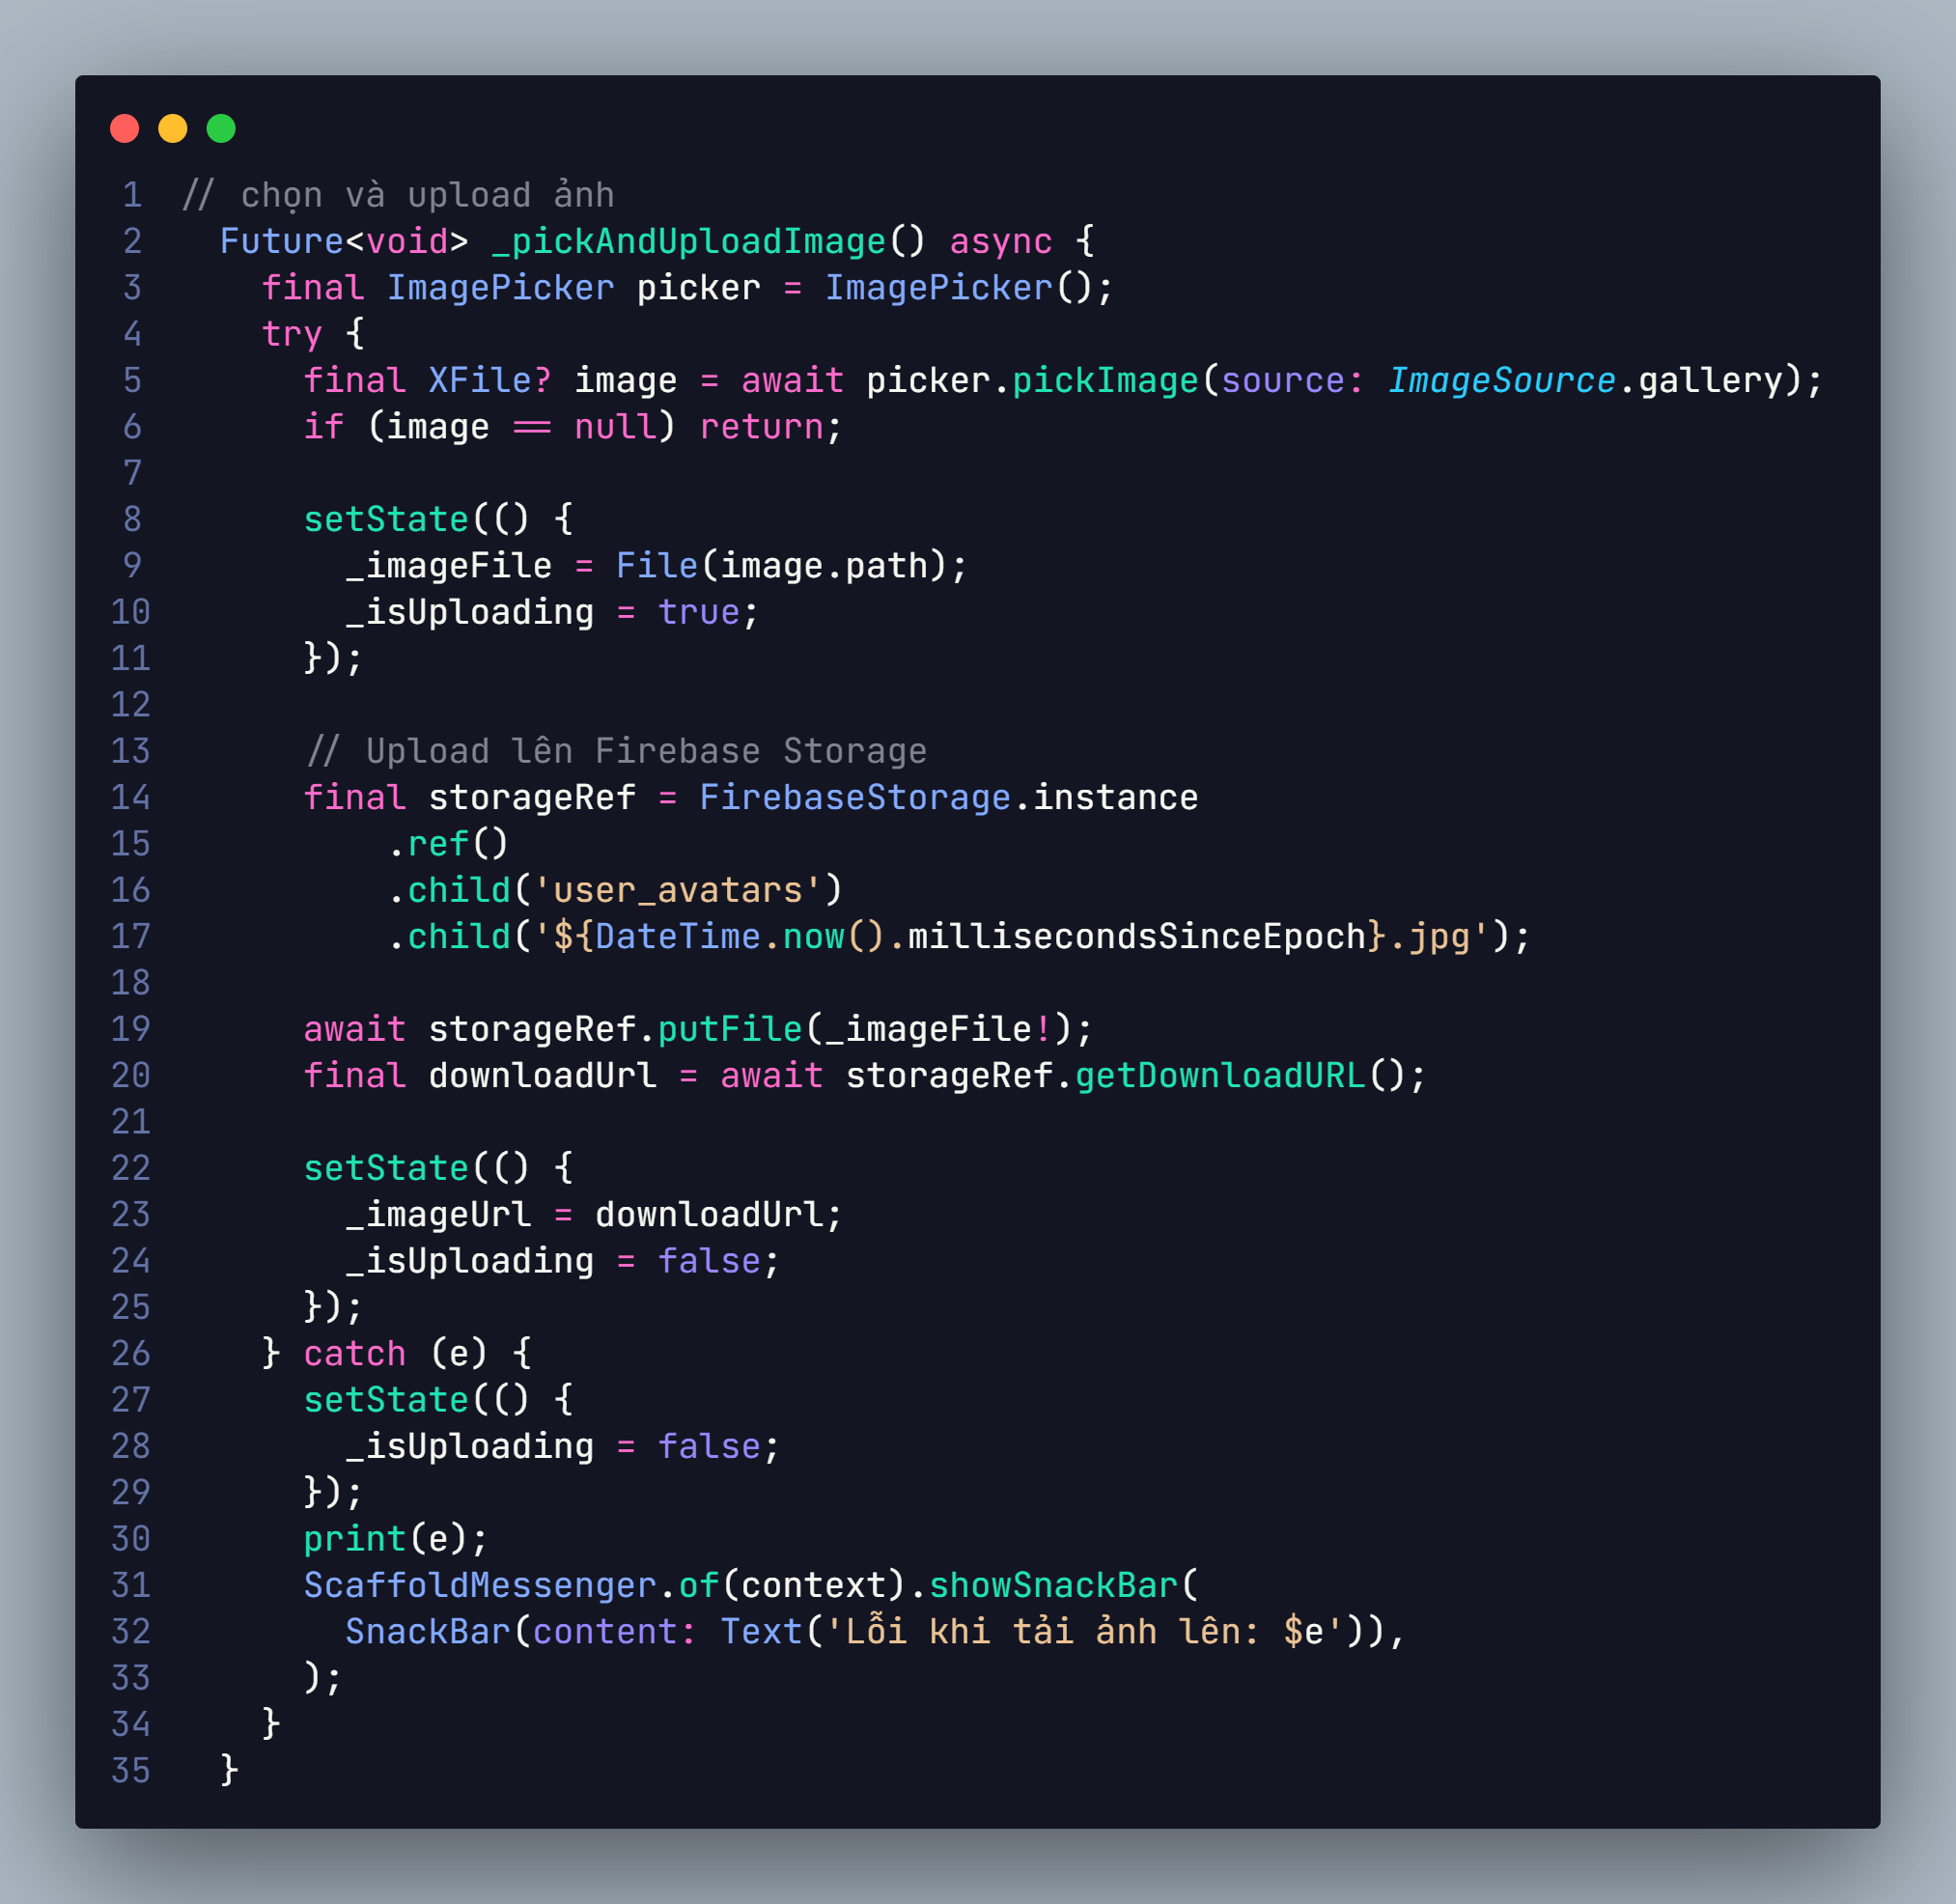
\includegraphics[width=0.8\textwidth]{Hinhve/Upload_anh_len_firebase.png}
  \caption{Tải hình ảnh lên Firebase}
  \label{fig:Upload_anh_len_firebase}
\end{figure}

\subsection{Kết quả}
\label{subsection:5.1.3}
Việc sử dụng Firebase Cloud Storage đã giúp đơn giản hóa việc lưu trữ hình ảnh, đơn giản hóa việc truyền tải và hiển thị ảnh và đồng thời giúp giảm dung lượng lưu trữ không cần thiết trong database.
Kết quả của việc sử dụng Firebase Cloud Storage và lưu các URL trong database được hiển thị như trong hình:
\begin{figure}[H]
  \centering
  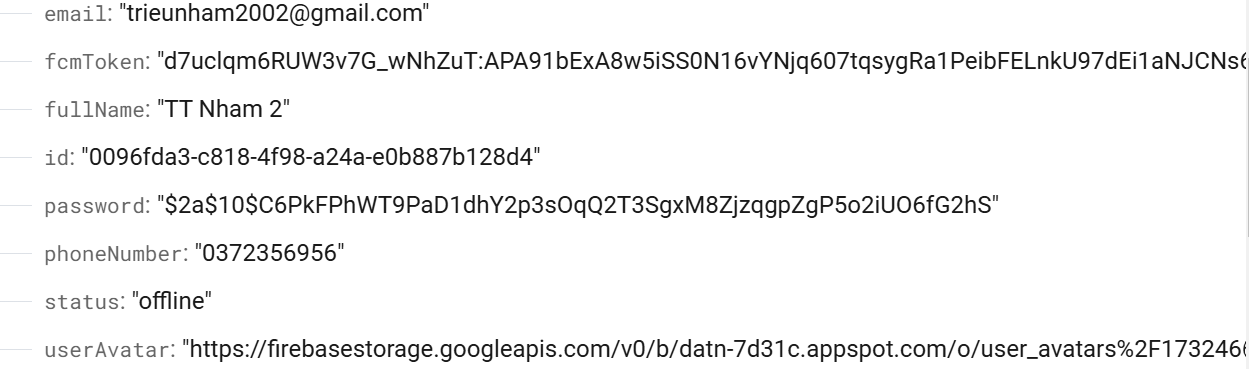
\includegraphics[width=0.8\textwidth]{Hinhve/Hien_thi_url_anh_firebase.png}
  \caption{Hiển thị URL hình ảnh trong database}
  \label{fig:Hien_thi_url_anh_firebase}
\end{figure}

\section{Thuật toán tính toán độ ưu tiên của tài xế khi thực hiện đặt xe}
\label{section:5.2}

\subsection{Vấn đề đặt ra}
\label{subsection:5.2.1}
Trong khi người dùng đặt chuyến xe, vào một thời điểm sẽ có nhiều tài xế đang hoạt động 
và có thể nhận chuyến xe. Do đó, cần phải có một thuật toán để tính toán tài xế tối ưu nhất để nhận chuyến xe đó.

\subsection{Giải pháp}
\label{subsection:5.2.2}
Để tính toán độ ưu tiên của tài xế, em dựa vào các thông tin như sau sau:
\begin{itemize}
  \item Đánh giá của tài xế (số sao).
  \item Khoảng cách mà tài xế đi đến địa điểm đón người đặt chuyến.
\end{itemize}

Trước hết để tính toán được khoảng cách mà tài xế đi đến địa điểm đón người đặt chuyến, em sử dụng công thức Haversine tính khoảng cách giữa hai điểm trên Trái Đất.
Việc tính toán khoảng cách được thực hiện như hình \ref{fig:Cong_thuc_Haversine}:
\begin{figure}[H]
  \centering
  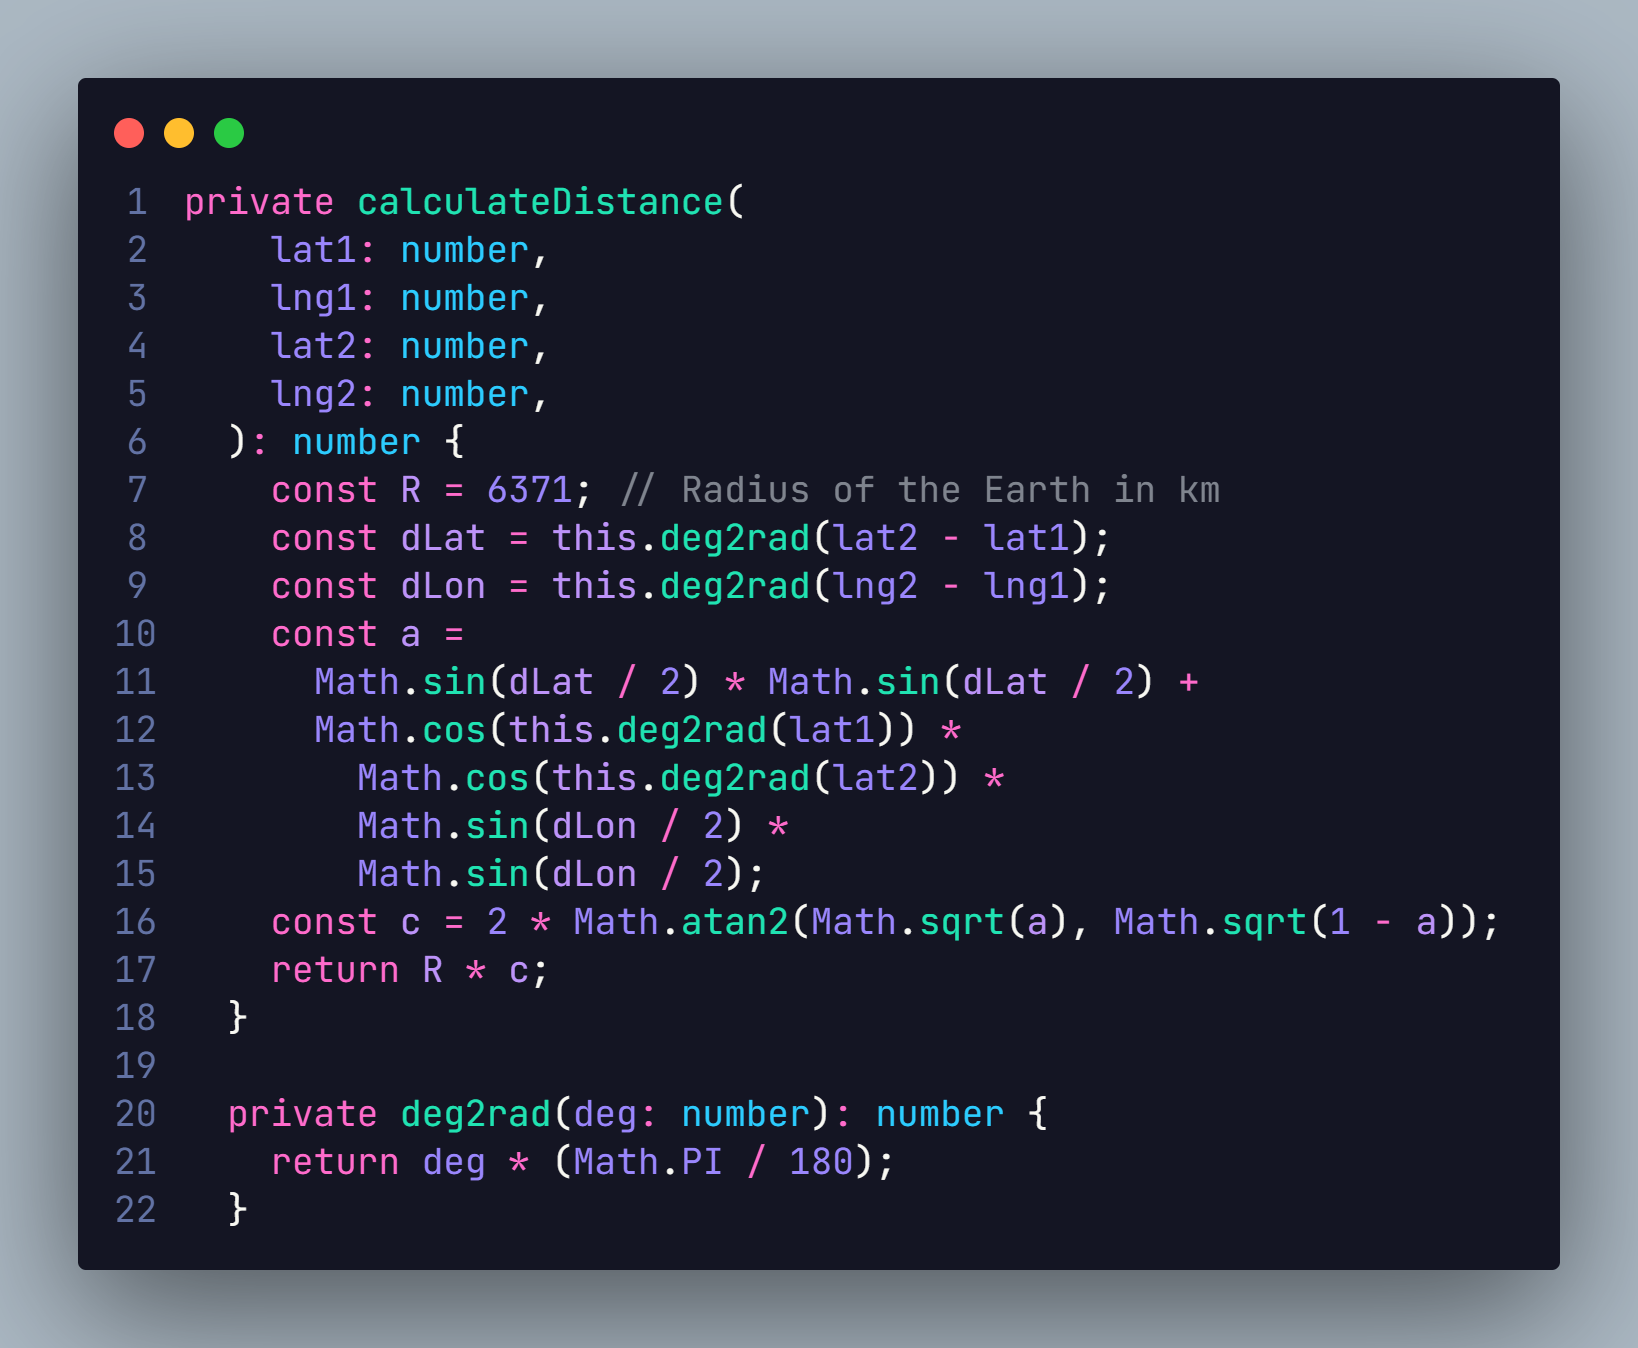
\includegraphics[width=0.8\textwidth]{Hinhve/Cong_thuc_Haversine.png}
  \caption{Công thức Haversine}
  \label{fig:Cong_thuc_Haversine}
\end{figure}
Sau khi tính toán được khoảng cách, em sẽ thực hiện việc chuẩn hóa và sắp xếp các tài xế theo độ ưu tiên.
Công việc trên được thể hiện như trong hình \ref{fig:Sap_xep_tai_xe_theo_do_uu_tien}: 
\begin{figure}[H]
  \centering
  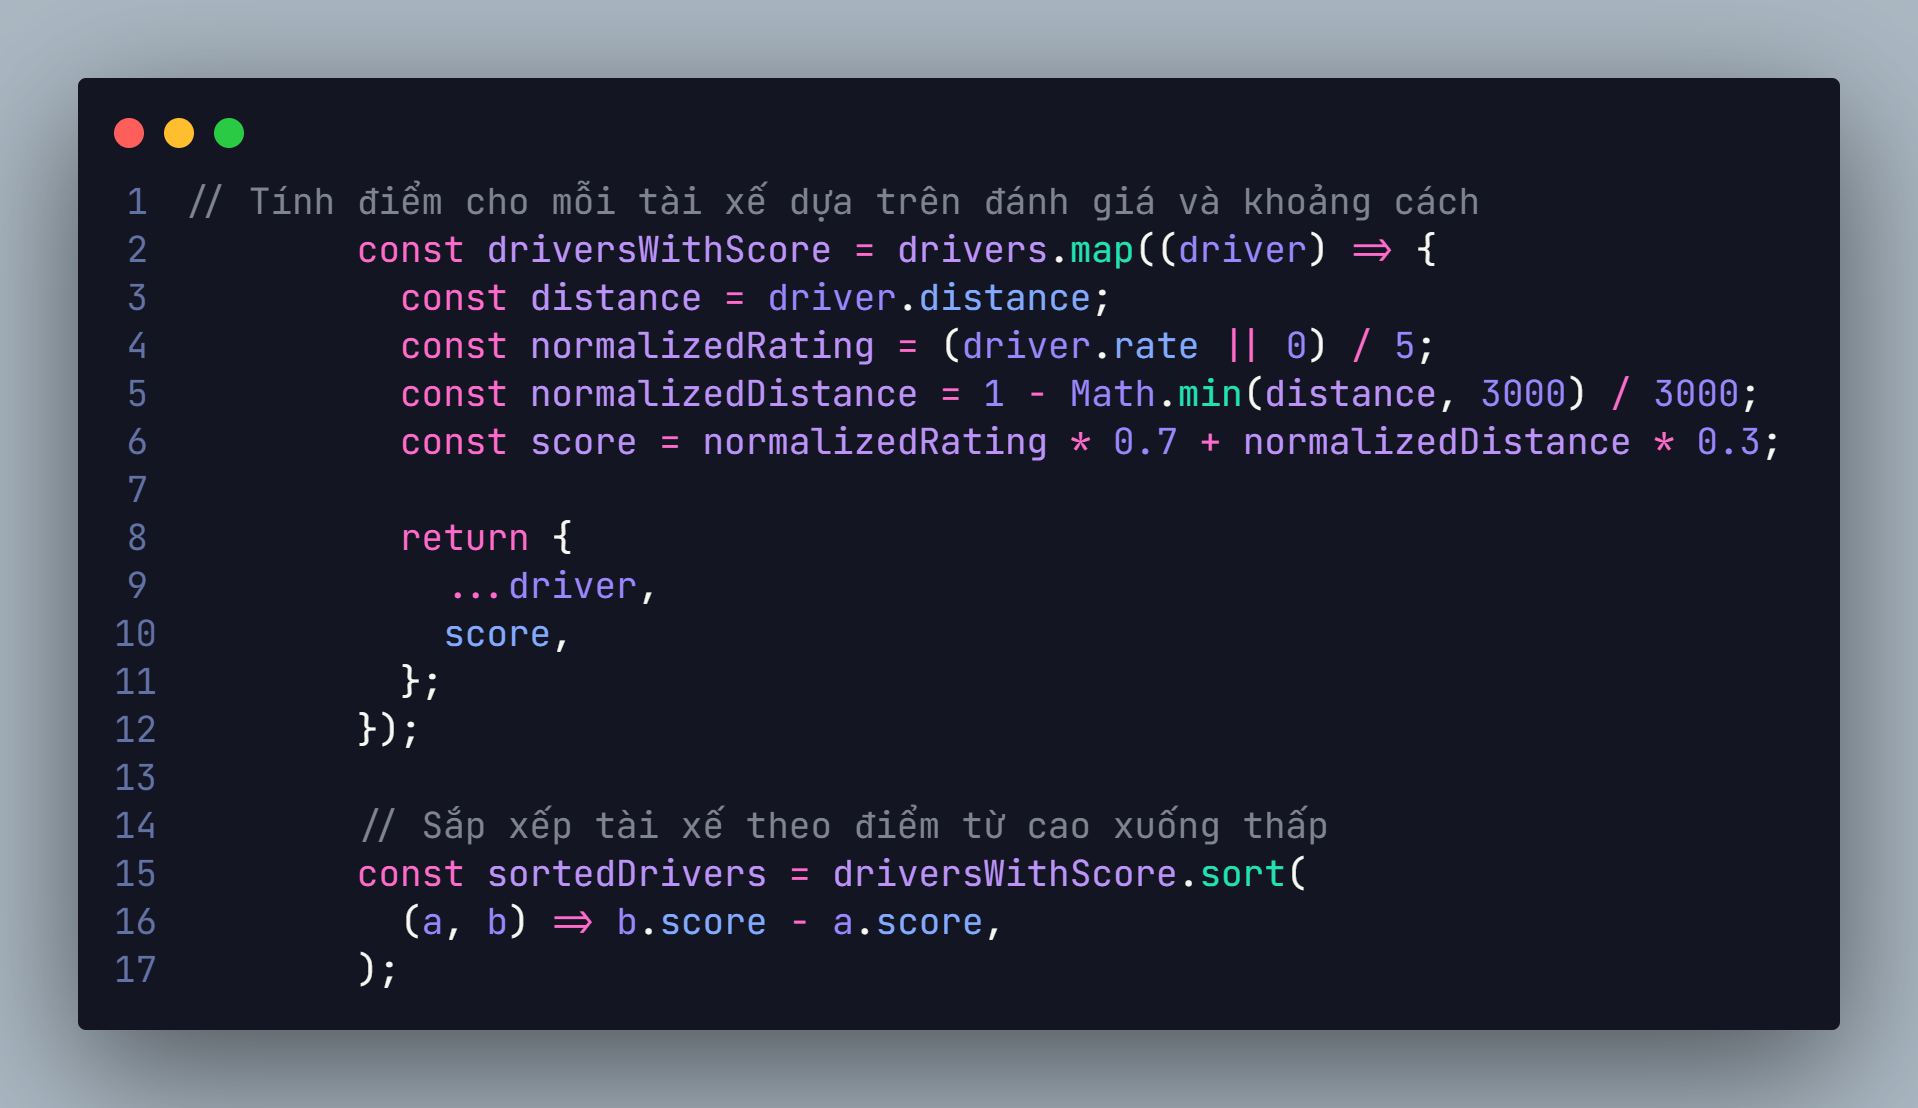
\includegraphics[width=0.8\textwidth]{Hinhve/Thu_tu_do_uu_tien.png}
  \caption{Sắp xếp các tài xế theo độ ưu tiên}
  \label{fig:Sap_xep_tai_xe_theo_do_uu_tien}
\end{figure}
\subsection{Kết quả}
\label{subsection:5.2.3}

Việc thực hiện tính toán khoảng cách và sắp xếp các tài xế theo độ ưu tiên đã giúp cho việc chọn tài xế phù hợp với mỗi người dùng, mỗi chuyến đi được chính xác hơn.
Giảm thiểu thời gian chờ đợi cho người đặt xe và tăng độ tin cậy trong việc lái xe.

\section{Theo dõi lịch trình di chuyển của tài xế}
\label{section:5.3}

\subsection{Vấn đề đặt ra}
\label{subsection:5.3.1}
Trong quá trình thực hiện chuyến đi, người dùng cần biết được vị trí hiện tại của tài xế để ước tính thời gian chờ đợi cũng như theo dõi hành trình di chuyển. Điều này đặc biệt quan trọng vì:
\begin{itemize}
  \item Giúp người dùng chủ động trong việc chuẩn bị và sắp xếp thời gian.
  \item Tăng tính minh bạch và độ tin cậy của dịch vụ.
  \item Đảm bảo an toàn cho cả người dùng và tài xế thông qua việc giám sát hành trình.
  \item Hỗ trợ việc giải quyết các khiếu nại hoặc tranh chấp nếu có phát sinh.
\end{itemize}

\subsection{Giải pháp}
\label{subsection:5.3.2}
Việc theo dõi vị trí được thực hiện ở cả 2 phía: người đặt xe và tài xế.

\textbf{Phía tài xế:} Ứng dụng sử dụng \texttt{Geolocator} để lấy vị trí với độ chính xác cao và đồng thời 
cập nhật liên tục vào Firebase Realtime Database bằng cách sử dụng \texttt{StreamBuilder}.

Hình \ref{fig:Theo_doi_vi_tri_tai_xe} minh họa việc theo dõi vị trí của tài xế:
\begin{figure}[H]
  \centering
  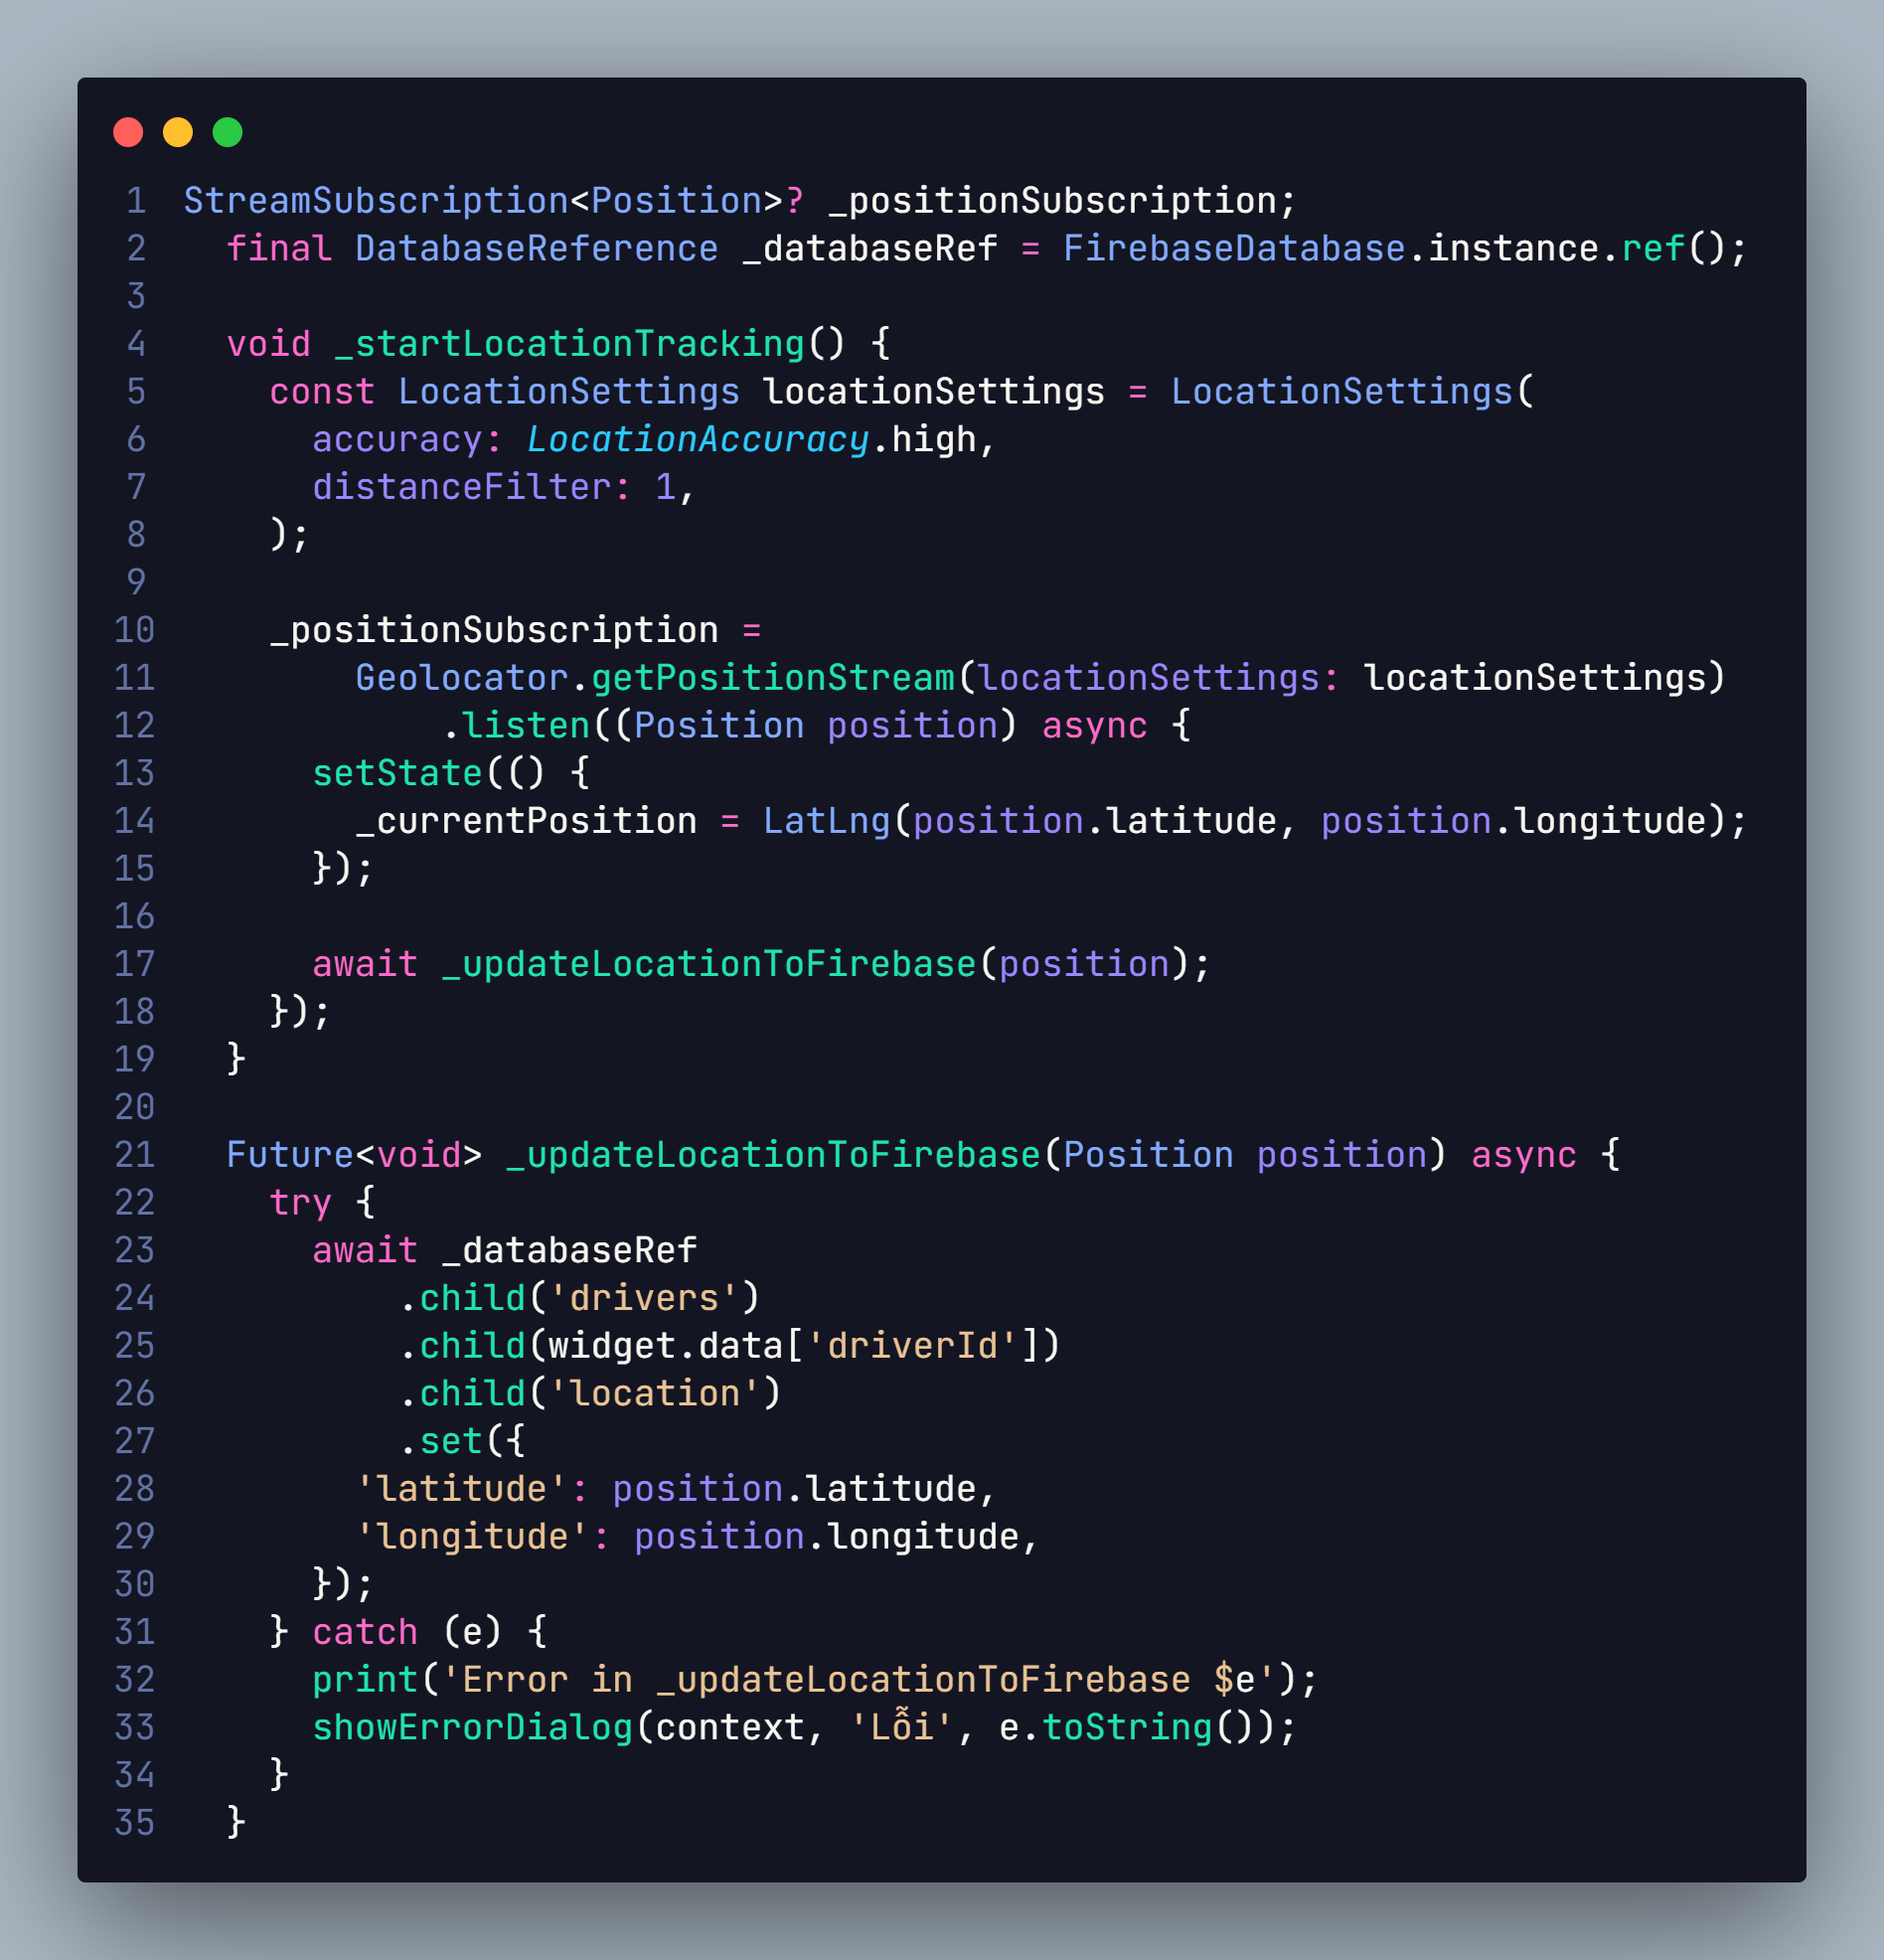
\includegraphics[width=0.8\textwidth]{Hinhve/Theo_doi_vi_tri_tai_xe.png}
  \caption{Cập nhật thay đổi vị trí của tài xế}
  \label{fig:Theo_doi_vi_tri_tai_xe}
\end{figure}

\textbf{Phía người đặt xe:} Ứng dụng lắng nghe sự thay đổi vị trí của tài xế từ Firebase Realtime Database và cập nhật thay đổi lên giao diện bản đồ của người dùng.

Hình \ref{fig:Theo_doi_vi_tri_nguoi_dat_xe} minh họa việc theo dõi vị trí của người đặt xe:
\begin{figure}[H]
  \centering
  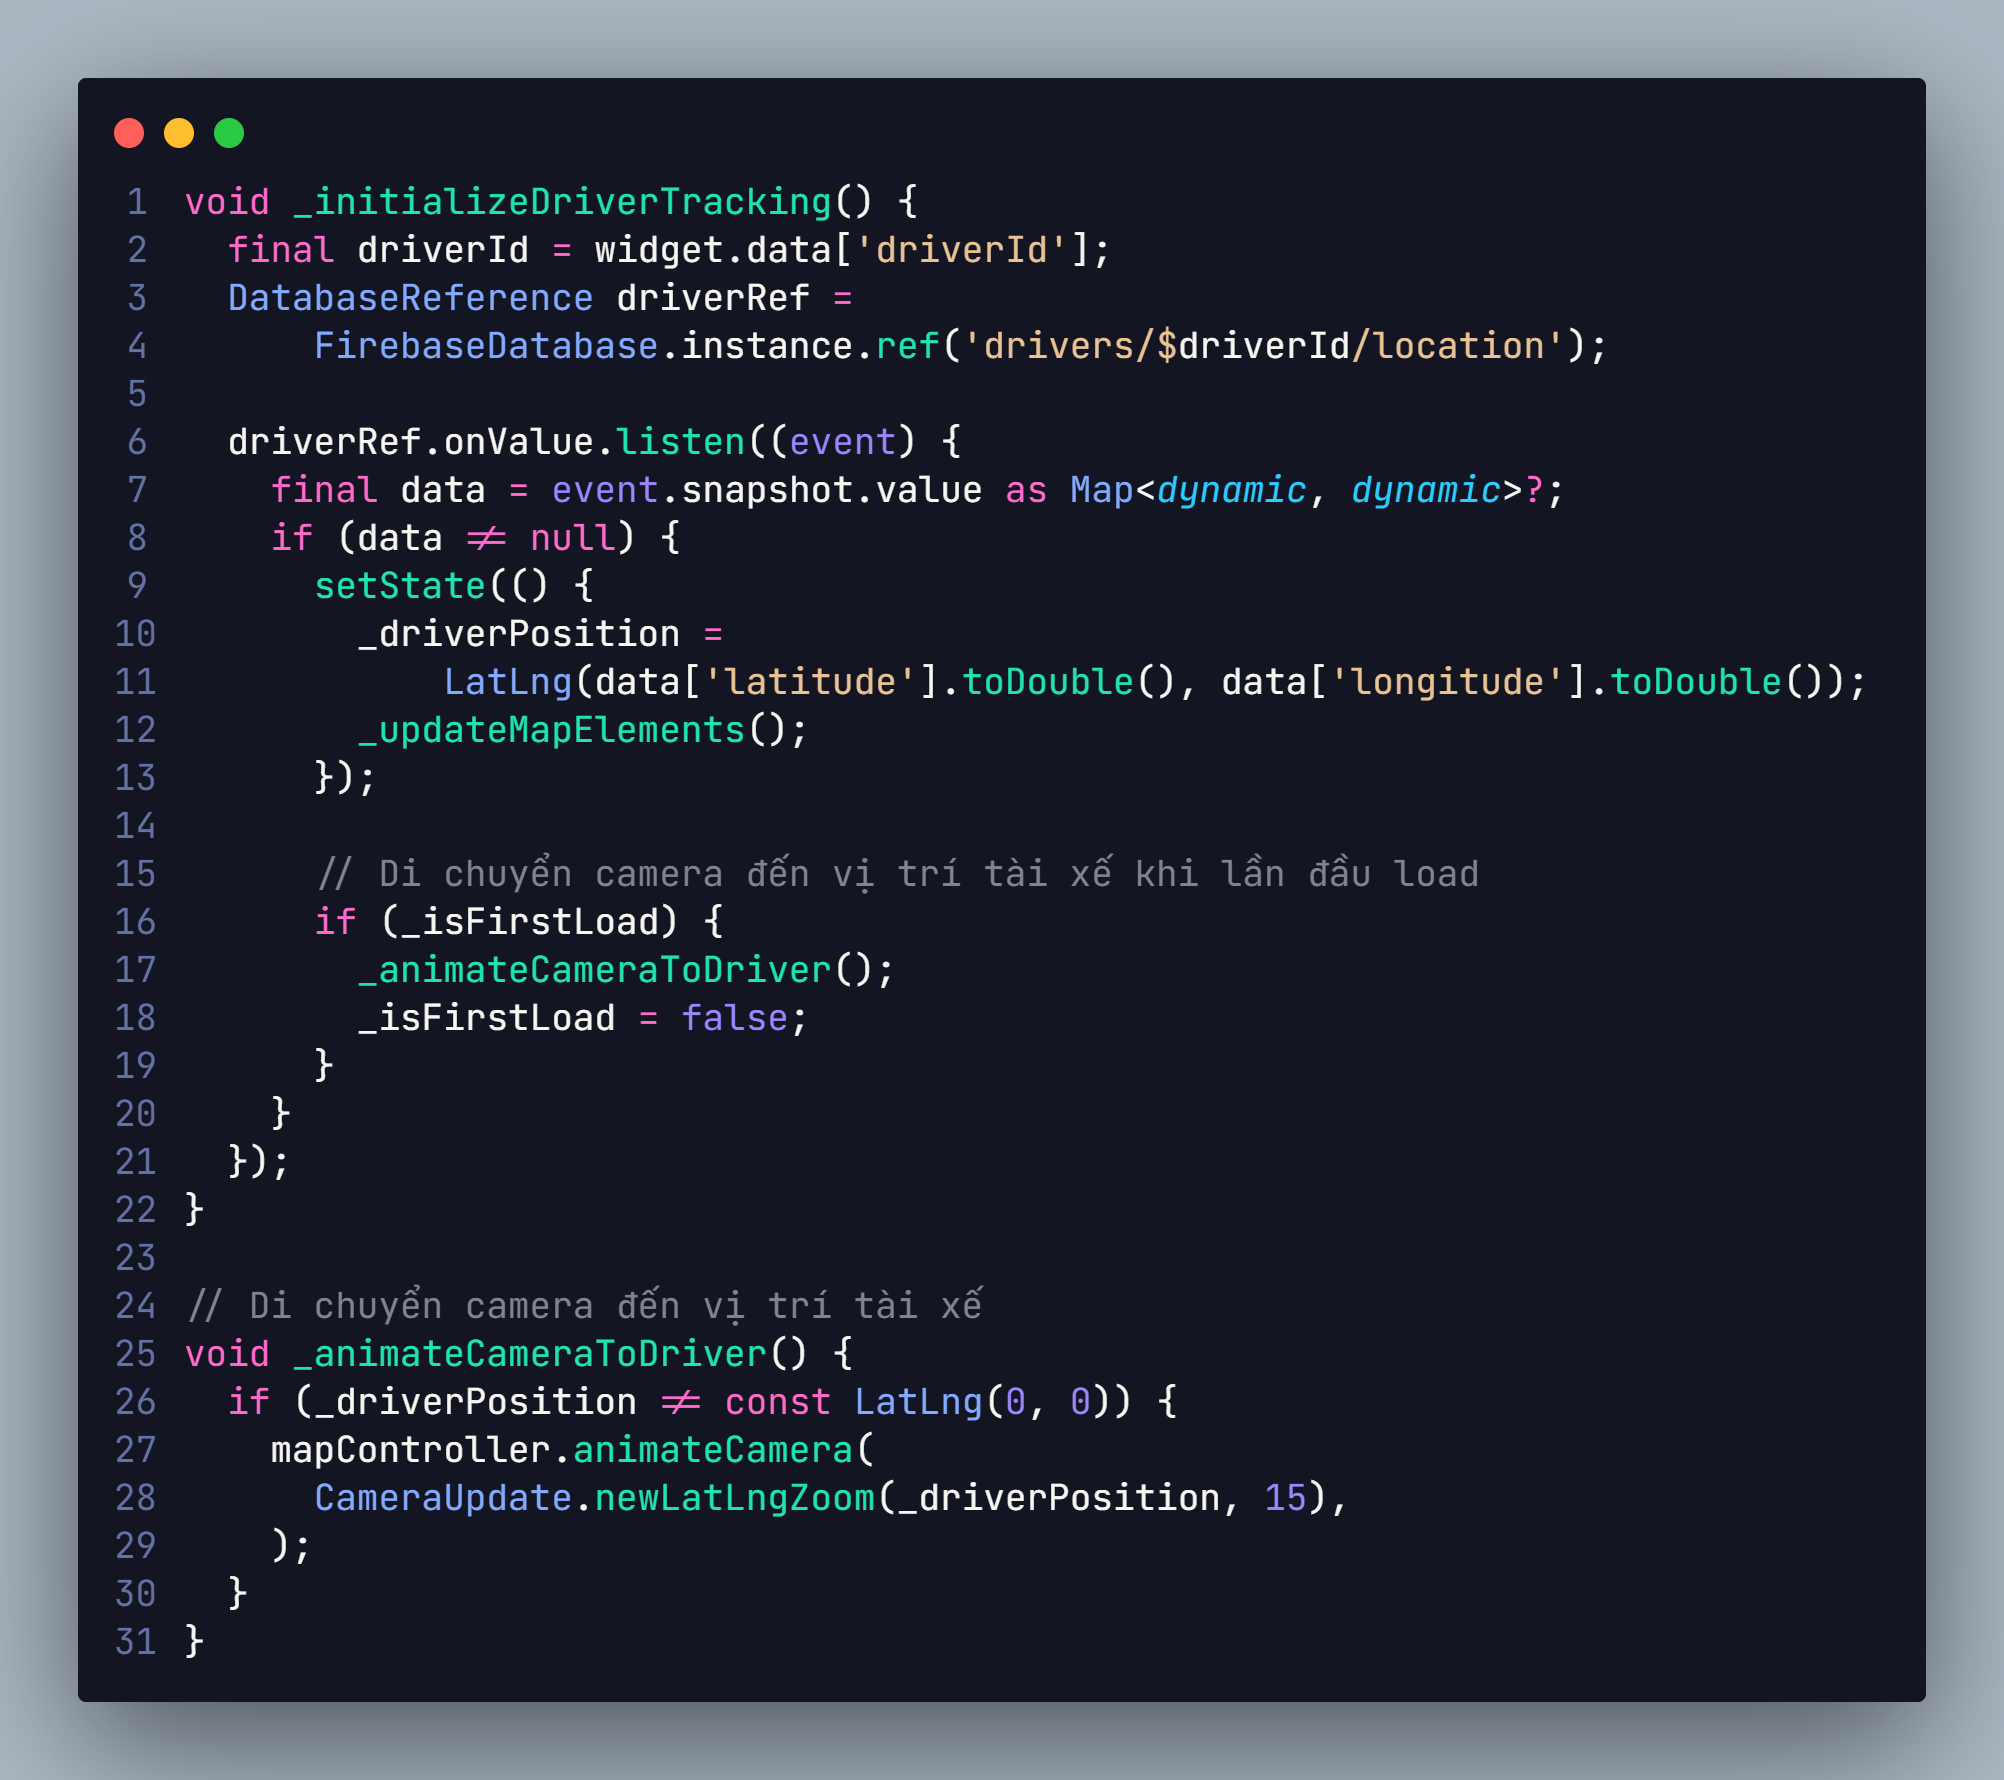
\includegraphics[width=0.8\textwidth]{Hinhve/Theo_doi_vi_tri_nguoi_dat_xe.png}
  \caption{Theo dõi vị trí di chuyển của tài xế}
  \label{fig:Theo_doi_vi_tri_nguoi_dat_xe}
\end{figure}

\subsection{Kết quả}
\label{subsection:5.3.3}
Như vậy, mỗi khi tài xế di chuyển ít nhất 1m thì vị trí của tài xế sẽ được cập nhật lên Firebase Realtime Database và người dùng sẽ được cập nhật vị trí mới này.

\section{Tính toán chi phí chuyến đi}
\label{section:5.4}

\subsection{Vấn đề đặt ra}
\label{subsection:5.4.1} 
Bên cạnh việc tính toán độ ưu tiên của tài xế, việc tính toán chi phí chuyến đi cũng là một vấn đề cần được giải quyết. 
Với chi phí hợp lý thì người dùng sẽ cảm thấy hài lòng và sẵn sàng sử dụng dịch vụ.

\subsection{Giải pháp}
\label{subsection:5.4.2}
Để tính toán chi phí chuyến đi một cách hợp lý, em đã xây công thức tính toán dựa trên các yếu tố sau:
\begin{itemize}
  \item Giá cước cơ bản (base fare): 20.000 VNĐ
  \item Giá theo kilomet: 5.000 VNĐ/km
  \item Phụ phí kẹt xe: 1.000 VNĐ/phút
  \item Phụ phí đêm khuya (23h - 5h sáng): 20.000 VNĐ
\end{itemize}

Quá trình tính toán được thực hiện thông qua các bước sau:
\begin{enumerate}
  \item Sử dụng Google Maps Directions API để lấy thông tin về:
  \begin{itemize}
    \item Khoảng cách giữa điểm đón và điểm đến
    \item Thời gian di chuyển dự kiến (có và không có kẹt xe)
    \item Đường đi chi tiết (polyline)
  \end{itemize}
  \item Tính toán chi phí cơ bản dựa trên khoảng cách
  \item Kiểm tra thời điểm đặt xe để tính phụ phí đêm khuya
  \item Tính toán phụ phí kẹt xe nếu thời gian di chuyển dự kiến vượt quá 50\% so với thời gian thông thường
\end{enumerate}

Hình \ref{fig:Tinh_toan_chi_phi} minh họa việc tính toán chi phí chuyến đi:
\begin{figure}[H]
  \centering
  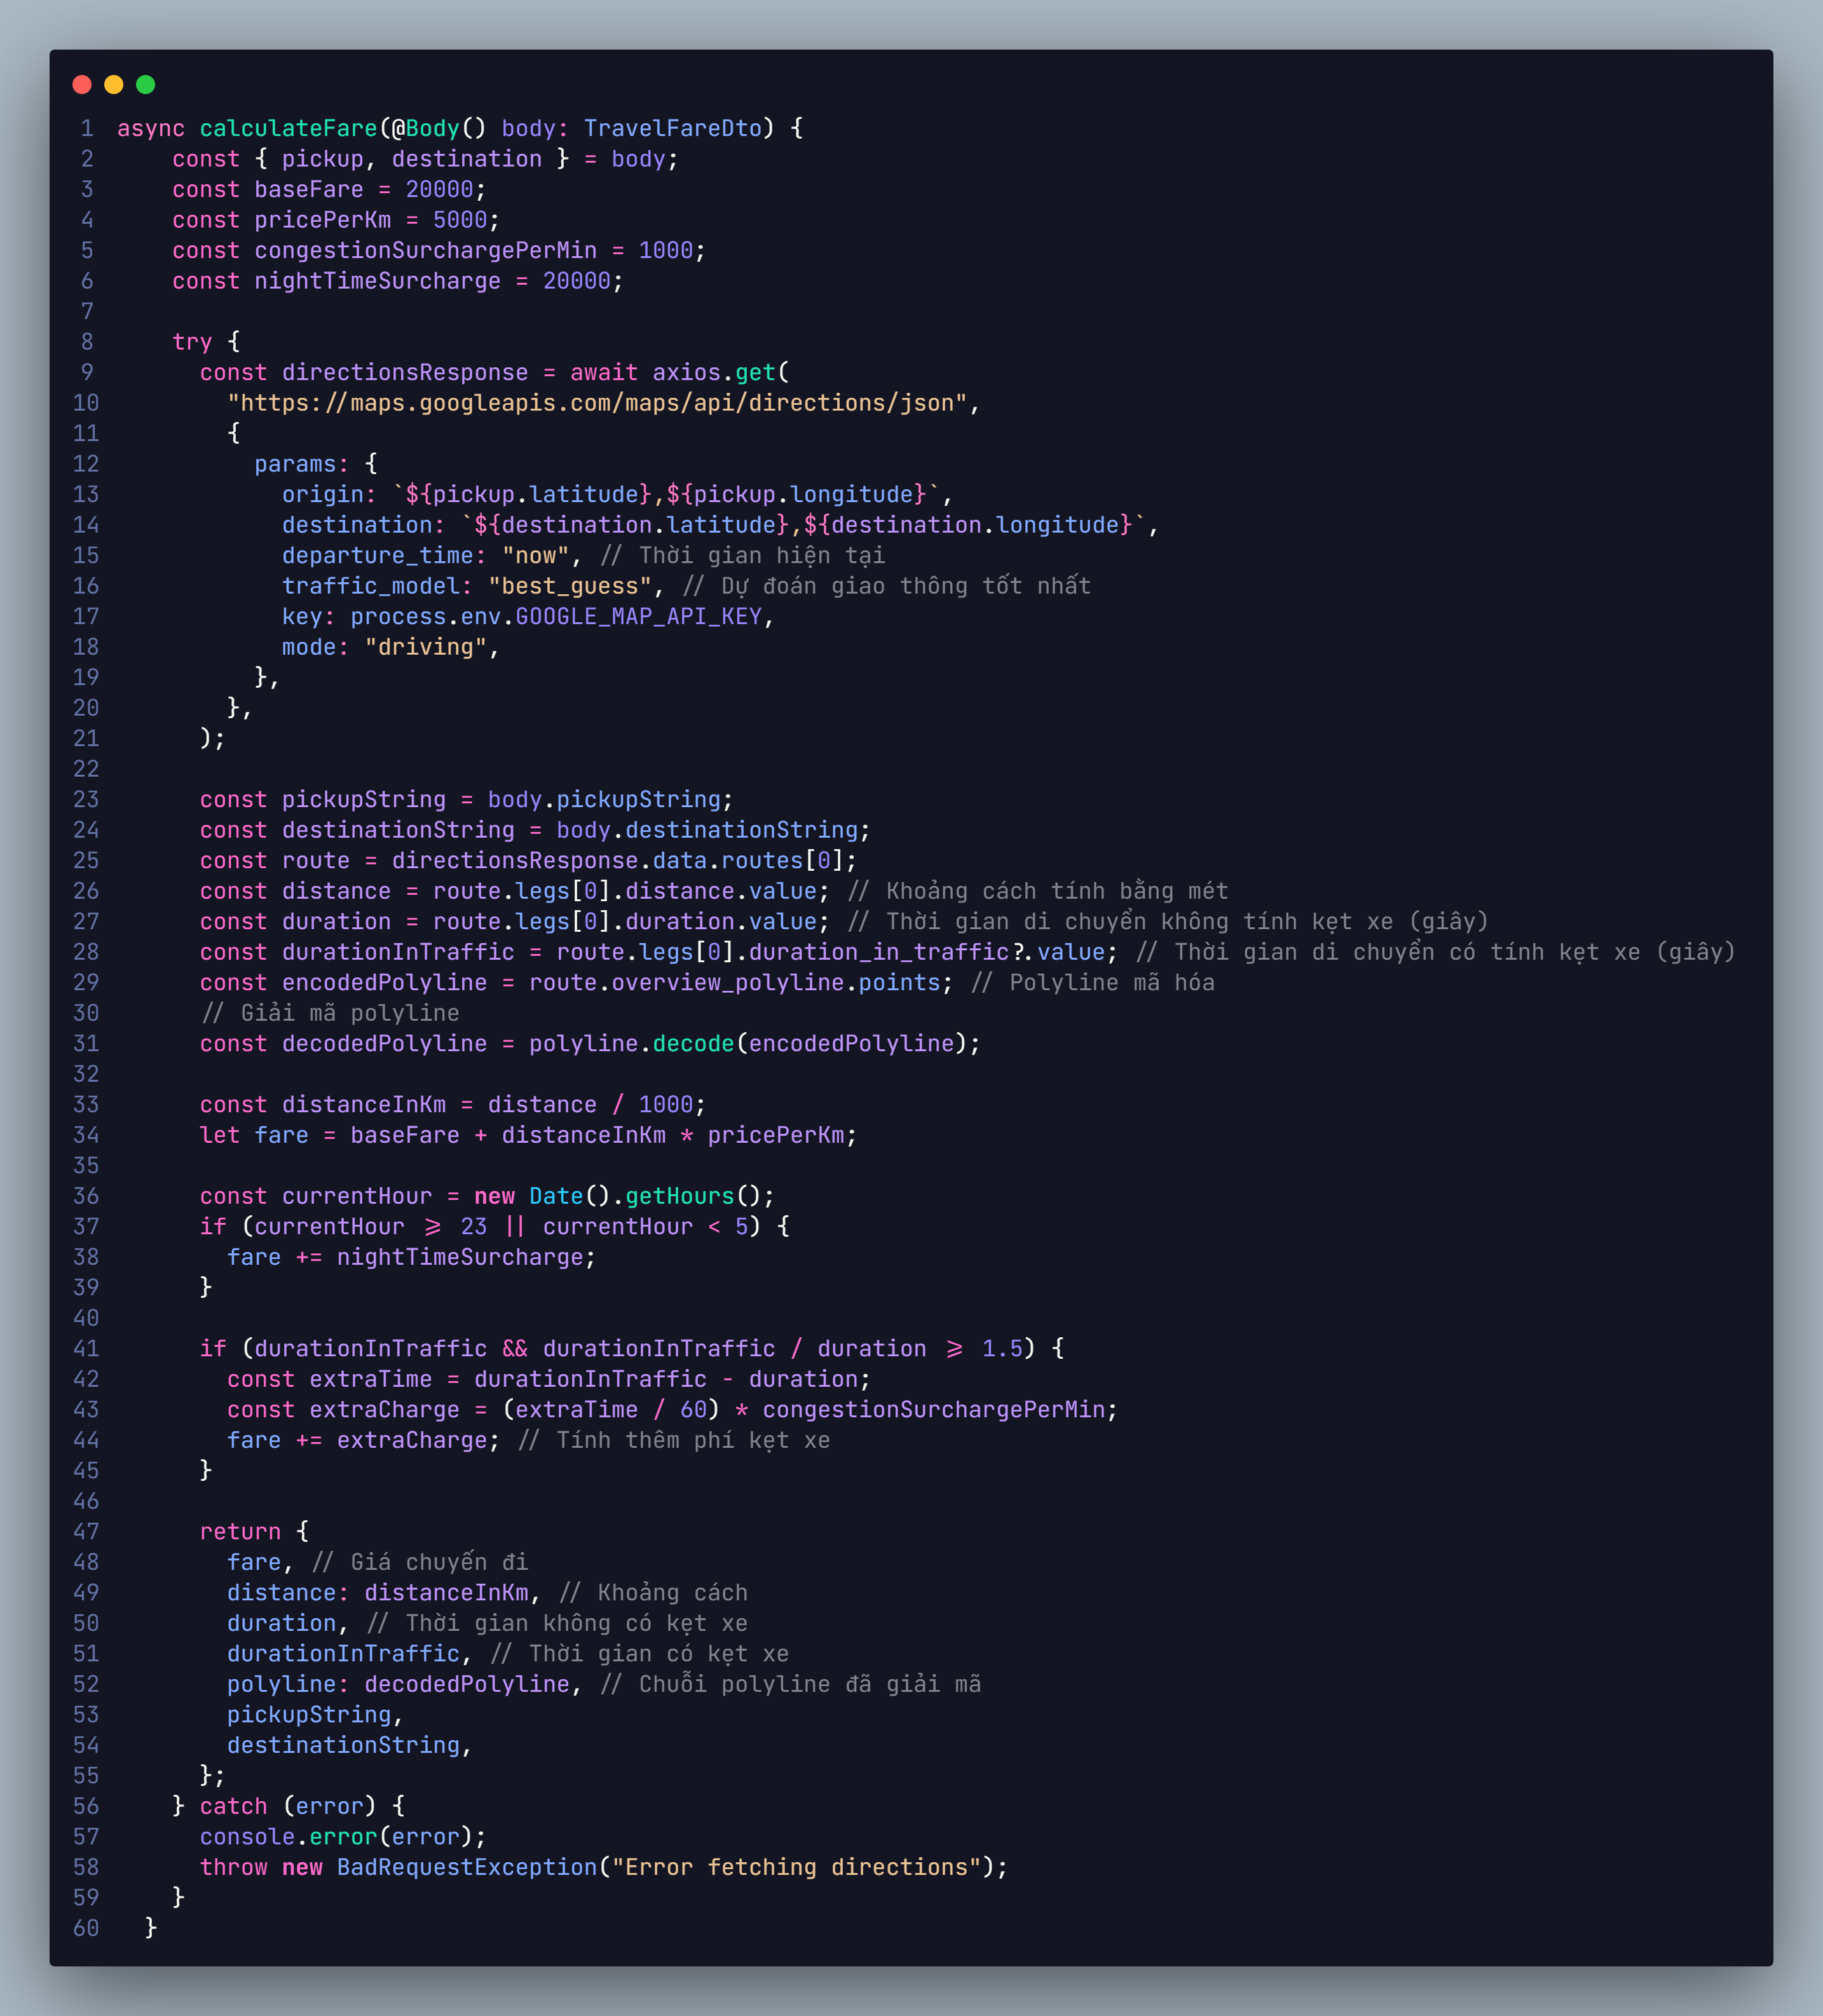
\includegraphics[width=0.8\textwidth]{Hinhve/Tinh_toan_chi_phi.png}
  \caption{Tính toán chi phí chuyến đi}
  \label{fig:Tinh_toan_chi_phi}
\end{figure}

\subsection{Kết quả}
\label{subsection:5.4.3}
Thuật toán tính chi phí đã mang lại những kết quả tích cực:
\begin{itemize}
  \item Chi phí được tính toán minh bạch, dựa trên các yếu tố thực tế
  \item Người dùng được thông báo chi phí trước khi bắt đầu chuyến đi
  \item Phụ phí kẹt xe và đêm khuya được tính hợp lý, phản ánh đúng điều kiện thực tế
  \item Tính toán được thực hiện tự động và chính xác nhờ tích hợp với Google Maps API
\end{itemize}

\end{document}